\documentclass[10pt,letterpaper]{article}
\usepackage[margin=1in]{geometry}
\usepackage[T1]{fontenc}
\usepackage{booktabs,graphicx,amsmath,hyperref}
\usepackage{longtable,float}
\title{S1 Appendix\\Coevolutionary balance of resting-state brain networks in autism}
\author{S. Rezaei Afshar and G. R. Jafari}
\date{Revision, October 27, 2026}
\begin{document}
\maketitle
\noindent This supplement accompanies the corrected revision analysis. The main Methods distinguish downloaded PCP fALFF derivatives from local regional aggregation and describe the limits of upstream documentation.
S2 Data contains the full machine-readable results; tables here summarize selected checks.
\renewcommand{\thetable}{S\arabic{table}}
\renewcommand{\thefigure}{S\arabic{figure}}

\section*{Cohort, coverage, and cortical assignment}
The original requested pool has 182 participants (90 ASD/92 controls). Age 18--30
and observed FIQ $>80$ yield 140 (69/71). This revision does not reconstruct a
randomly sampled 100/100 cohort. All available participants were recorded male;
handedness is not an exclusion. Technical exclusions diagnosed with all 200
parcels in Stage 1 are not automatically carried into the primary 106-node design;
all primary participants must instead satisfy the frozen selected-node QC rule.

The primary model omits CMU ($n=1$ ASD), SBL ($n=1$ ASD), and UM\_2 ($n=2$
controls) under the site-size rule, leaving 136 (67/69). Broader-181 and full-200
feature cohorts contain 104 (48/56) and 69 (31/38), and their adjusted models
contain 101 (47/54) and 64 (30/34). Full per-design and trimming manifests are
included in S2 Data.

Of the primary 106 nodes, 13 are visual, 16 somatomotor, nine dorsal attention,
24 salience/ventral attention, one limbic, 14 frontoparietal, 14 default, and 15
unassigned. Global quantities retain all 106; cortical block sums omit edges
involving unassigned nodes. A within-limbic pair does not exist. Three
within-limbic quantities and the legacy bipolarity descriptor are unavailable or
excluded from the 88-feature inferential schema. The same schema, including
both graph efficiencies, is used in both pipelines for clinical and predictive
analyses. The complete ROI list and assignment table are provided in S2.

Table~\ref{tab:Ssites} gives the primary model site-by-diagnosis counts.
\begin{table}[htbp]
\centering
\small
\caption{Primary adjusted-model site counts. CALTECH contributes only ASD participants.}\label{tab:Ssites}
\begin{tabular}{lrr}
\toprule
SITE\_ID & ASD & Control \\
\midrule
CALTECH & 9 & 0 \\
LEUVEN\_1 & 11 & 5 \\
MAX\_MUN & 5 & 12 \\
NYU & 12 & 19 \\
OLIN & 4 & 3 \\
PITT & 4 & 8 \\
TRINITY & 7 & 7 \\
UM\_1 & 1 & 2 \\
USM & 14 & 13 \\
\bottomrule
\end{tabular}
\end{table}


\section*{Site diagnostics and restricted sensitivity}
For each design and pipeline, the original adjusted-model participant list is
joined to saved raw and ComBat feature exports. The model matrix contains an
intercept, diagnosis, standardized age, FIQ, FD, and site indicators. All designs
have full rank. Site partial $R^2$ is
$(\mathrm{SSE}_{\mathrm{without\ site}}-\mathrm{SSE}_{\mathrm{with\ site}})/
\mathrm{SSE}_{\mathrm{without\ site}}$. It describes the additional fit attributable
to site under this model. Median-centered Levene statistics compare biological-
covariate residual dispersion across sites. These post-ComBat summaries are
exploratory descriptive diagnostics on the fitting sample, not independent tests
that harmonization succeeded. No diagnostic flag triggers participant removal.
The main manuscript now retains dedicated within-network and between-network
Results sections and full cortical effect figures. Gray cells are structurally
unavailable; no primary cortical test survives its family correction.
the supporting figures below displays the exact residualized global-efficiency
comparisons underlying the saved partial correlations.

Raw primary maximum Cook's distance is .080 with GSR and .062 without GSR;
maximum leverage is .352. HC3 uncertainty accounts for leverage but does not
supply site-clustered inference. Influence records, site/group H summaries, and
all diagnostic values are retained in S2 Data.

The mixed-diagnosis-site restriction excludes CALTECH's nine ASD participants,
leaving 127 participants (58 ASD and 69 controls) at eight sites. Adjusted
coefficients are 1.115 (95\% CI $-17.531$, 19.762) with GSR and 1.660
($-12.775$, 16.096) without GSR; both Holm $p=1$. Larger-node models already
contain only mixed-diagnosis sites and therefore retain their original estimates.
This is a raw adjusted sensitivity; we do not refit ComBat in the restricted cohort.

Table~\ref{tab:Sdiag} summarizes the primary site and influence diagnostics.
\begin{table}[htbp]
\centering
\small
\caption{Primary-model diagnostics. Site partial $R^2$ is descriptive and conditional on diagnosis, age, FIQ and mean FD. The design is identical before and after ComBat.}\label{tab:Sdiag}
\begin{tabular}{llrrr}
\toprule
Pipeline & Version & Site partial R2 & Max leverage & Max Cook's D \\
\midrule
GSR & raw & 0.056 & 0.352 & 0.080 \\
GSR & ComBat & 0.004 & 0.352 & 0.079 \\
noGSR & raw & 0.047 & 0.352 & 0.062 \\
noGSR & ComBat & 0.005 & 0.352 & 0.072 \\
\bottomrule
\end{tabular}
\end{table}


\section*{Node-set sensitivities}
the supporting figures below shows raw adjusted Hamiltonian coefficients. Each design has
its own participant set and total edge count. Raw energy magnitudes are therefore
not interchangeable across designs. Complete estimates for ComBat and pooled
trimming, including participant-specific exclusions and trimming fences, are
in S2 Data. No corrected diagnosis effect is detected in these
models; sensitivity agreement does not demonstrate equivalence.


\section*{Original-analysis continuity and H--metric complements}
The original manuscript distinguishes global, within-network, between-network,
within-group H relationships, clinical Pearson/Spearman correlations, PLSR,
PLSC, and classification, with GSR/no-GSR sensitivity. These questions are now
again named explicitly in the main Results. The complete original-to-revision
map, significant association lists, nominal-only group results, and original
export reproduction checks are included under continuity/ in S2.

All 364 original exported H--feature Pearson correlations, raw probabilities and
per-group FDR probabilities were reproduced numerically from the supplied original
feature tables to absolute tolerance $10^{-10}$. The original no-GSR ASD
H--global-efficiency association is $r=-.324338$, $p=.003334$, $q=.005917$
($n=80$). It is therefore present in those original data. That source sample and
feature construction differ from the revised common-node analysis; replication
of an export is not confirmation of the exact submitted run or proof of a group
interaction. The revised raw-eligible correlations use 69 ASD and 71 controls,
whereas matched raw/ComBat complements use 67 and 69.

Table~\ref{tab:SHmatched} reports both matched versions, including nonsignificant
blocks. The 348-test alternative pools diagnosis/pipeline blocks; it can change
a subgroup's q-values in either direction and is not described as uniformly
stricter. Shared Hamiltonian/block terms and proportional weighted-FC/energy
features mean significant counts are not independent biological discoveries.
The original negative efficiency association is not recovered in the revised
raw eligible feature definition, independently of nuisance adjustment.

\begin{table}[htbp]
\centering\small
\caption{Descriptive Pearson H associations on identical model participants before/after ComBat. q87 uses per-group correction; q348 pools all four pipeline/group blocks per version. Neither correction scope is uniformly more conservative for every subgroup.}\label{tab:SHmatched}
\begin{tabular}{lllrrr}
\toprule
Version & Pipeline & Group & N & q87<.05 & q348<.05 \\
\midrule
ComBat matched & GSR & ASD & 67 & 24 & 22 \\
ComBat matched & GSR & Control & 69 & 25 & 18 \\
ComBat matched & noGSR & ASD & 67 & 10 & 10 \\
ComBat matched & noGSR & Control & 69 & 0 & 10 \\
Raw matched & GSR & ASD & 67 & 28 & 18 \\
Raw matched & GSR & Control & 69 & 19 & 19 \\
Raw matched & noGSR & ASD & 67 & 10 & 12 \\
Raw matched & noGSR & Control & 69 & 0 & 6 \\
\bottomrule
\end{tabular}
\end{table}


Table~\ref{tab:Slegacy} reports the original spectral descriptor as a separate
exploratory raw adjusted sensitivity. Its two tests are Holm corrected separately
from the frozen primary/secondary families; it remains absent from clinical and
prediction feature schemas. Both adjusted probabilities are .916.

\begin{table}[htbp]
\centering\small
\caption{Original spectral bipolarity descriptor: additional exploratory raw adjusted diagnosis models. Holm covers the two pipeline tests, separately from the frozen inferential families. The descriptor is not asserted to optimize signed structural balance.}\label{tab:Slegacy}
\begin{tabular}{lrlllr}
\toprule
Pipeline & N & Coefficient & CI low & CI high & Holm p \\
\midrule
GSR & 136 & 0.0004 & -0.0067 & 0.0075 & 0.916 \\
noGSR & 136 & 0.0105 & -0.0175 & 0.0386 & 0.916 \\
\bottomrule
\end{tabular}
\end{table}


Table~\ref{tab:Sbothnull} retains the original null-model question in both diagnostic
groups. These individual tests use a pooled 560-comparison exploratory BH family;
the separate 71-control baseline retains its explicit 284-comparison correction.
Neither family tests an ASD--control difference in H or null z.

\begin{table}[htbp]
\centering\small
\caption{Separate diagnostic-group summaries of the existing state-permutation nulls. Exploratory BH covers all 560 participant/pipeline/null comparisons here. Control-only 284-test correction is a different explicitly labeled family.}\label{tab:Sbothnull}
\begin{tabular}{lllrrr}
\toprule
Group & Pipeline & Null & N & Mean z & q<.05 count \\
\midrule
ASD & GSR & Blocked & 69 & -2.331 & 40 \\
ASD & GSR & Unrestricted & 69 & -4.705 & 61 \\
ASD & noGSR & Blocked & 69 & -2.591 & 46 \\
ASD & noGSR & Unrestricted & 69 & -4.917 & 60 \\
Control & GSR & Blocked & 71 & -2.313 & 36 \\
Control & GSR & Unrestricted & 71 & -4.690 & 61 \\
Control & noGSR & Blocked & 71 & -2.760 & 50 \\
Control & noGSR & Unrestricted & 71 & -5.159 & 64 \\
\bottomrule
\end{tabular}
\end{table}


\section*{Clinical analyses}
The five scores are ADI-R social ($n=30$), ADI-R verbal ($n=30$), ADI-R onset
($n=28$), ADOS total ($n=50$), and ADOS communication ($n=43$), identically across
pipelines. Negative/sentinel values are missing. Feature correlations use all
available 88 features. Adjusted Hamiltonian correlations use age, IQ, mean FD,
and site. No feature or adjusted Hamiltonian correlation survives its specified
BH correction. The ADOS and five-score complete-case PLSC blocks are exploratory;
rank-wise permutation probabilities across all reported latent variables are
BH corrected. A nominal no-GSR five-score LV3 $p=.00699$ becomes $q=.0979$.
All PLSC and correlation rows, including nonsignificant tests, are included in S2.
the supporting figures below displays all adjusted H correlations and OOF PLSR scores.
The prior loading figures came from superseded fitted models; they are not
reused as current component estimates.

Table~\ref{tab:Splsr} lists every score-specific PLSR validation result.
\begin{table}[htbp]
\centering
\small
\caption{Nested site-held-out PLS regression. Baselines predict the outer-fold training mean. Negative OOF $R^2$ does not imply evidence of an inverse biological effect.}\label{tab:Splsr}
\begin{tabular}{llrrrr}
\toprule
Pipeline & Score & N & OOF R2 & OOF MSE & Baseline MSE \\
\midrule
GSR & ADI R Social & 30 & -0.416 & 37.895 & 27.874 \\
GSR & ADI R Verbal & 30 & -0.130 & 25.895 & 23.572 \\
GSR & ADI R Onset & 28 & -0.928 & 3.512 & 2.017 \\
GSR & ADOS Total & 50 & -0.029 & 10.838 & 10.723 \\
GSR & ADOS Communication & 43 & -0.047 & 1.409 & 1.392 \\
noGSR & ADI R Social & 30 & -0.381 & 36.939 & 27.874 \\
noGSR & ADI R Verbal & 30 & -0.370 & 31.387 & 23.572 \\
noGSR & ADI R Onset & 28 & -0.348 & 2.455 & 2.017 \\
noGSR & ADOS Total & 50 & -0.105 & 11.633 & 10.723 \\
noGSR & ADOS Communication & 43 & -0.305 & 1.756 & 1.392 \\
\bottomrule
\end{tabular}
\end{table}


\section*{Male-control null baseline reported separately}
All 71 eligible male controls from nine sites are included in this baseline,
including controls at sites too small for the group regression. No energy-based
trimming is applied. For each of the two pipelines and two state-permutation
schemes there are exactly 71 distinct control records (284 comparisons total).
Each record retains the original 1,000-permutation Monte Carlo probability.
An exploratory BH correction spans all 284 individual comparisons. The counts
of lower-tail $p<.05$ are 64/69 for unrestricted GSR/no-GSR and 40/53 for blocked
GSR/no-GSR; the corresponding BH $q<.05$ counts are 61/64 and 36/50.
These counts do not test ASD versus controls.

Mean control $z$ is $-4.690$ with GSR and $-5.159$ without GSR for unrestricted
states, versus $-2.313$ and $-2.760$ within network/hemisphere blocks.
the supporting figures below displays every control's score. Mean empirical-minus-null
energy intervals resample sites 5,000 times (seed 20261026), computing the
participant-weighted mean in each resampled set of whole site clusters. The
percentile intervals condition on the saved null means and do not include all
Monte Carlo estimation uncertainty or constitute a pooled randomization test.
S2 contains the complete control-only table and all interval endpoints.

These null configurations hold each participant's full signed weighted FC matrix
fixed and randomize only state assignment. They address whether observed relative
fALFF states align with that FC more than randomized states do. They do not test
against degree-rewired or signed-weight-shuffled networks. The two latter nulls
would ask additional questions and are not claimed to have been run here.

\section*{Randomization and mathematical coupling}
Unrestricted permutations preserve FC and the total number of nodal labels.
Network/hemisphere permutations additionally preserve state counts within the
specified blocks. Their lower-tail probabilities test alignment under those
randomizations, not an autism group effect. Small blocks may offer few distinct
permutations, and neither scheme preserves full spatial autocorrelation. No
primary participant has zero null variance. The participant records include the
number of positive states, observed energy, null mean/SD, Monte Carlo probability,
and the coefficient linking a uniform weight shift to energy.

For $n$ nodes with $s_i\in\{-1,+1\}$,
$\sum_{i<j}s_i s_j=((\sum_i s_i)^2-n)/2$. Thus adding a constant $c$ to each
Fisher weight changes $H$ by $[n-(\sum_i s_i)^2]c/2$. With 53 positive and
53 negative labels the coefficient is 53, rather than the 100 appropriate to
exactly balanced 200-node states. Median ties can change that coefficient and
are not forced into artificial equal halves.

Table~\ref{tab:Snull} summarizes both diagnosis groups together; the control-only
baseline above is reported separately.
\begin{table}[htbp]
\centering
\small
\caption{Descriptive participant null-score summaries. These are alignment randomizations, not diagnostic tests or full spatial-autocorrelation nulls.}\label{tab:Snull}
\begin{tabular}{llrrr}
\toprule
Pipeline & Null & N & Mean z & SD z \\
\midrule
GSR & Network/hemisphere & 140 & -2.322 & 1.449 \\
GSR & Unrestricted & 140 & -4.698 & 2.480 \\
noGSR & Network/hemisphere & 140 & -2.677 & 1.631 \\
noGSR & Unrestricted & 140 & -5.039 & 2.432 \\
\bottomrule
\end{tabular}
\end{table}


\section*{Prediction and reproducibility}
Outer classification folds have 31, 28, 27, 27, and 27 participants. Sites are
disjoint between train and test; both classes are present in every inner and
outer split. All 10 completed classifier/pipeline pairs have predictions for all 140
participants. Hyperparameter selection is restricted to inner folds, and ComBat
is not used. Feature availability and node QC are cohort-wide, limiting the
analysis to exploratory prediction conditional on the fixed feature schema.
OOF intervals bootstrap sites from fixed predictions; they do not repeatedly
refit the complete training and QC process.
the supporting figures below use all 140 OOF predictions for
each model and pipeline. No best classifier is selected using those plots;
pooled ROC curves remain descriptive in this site-held-out setting.

% CLASSIFICATION_SUPPLEMENT_BEGIN
The original-algorithm extension currently covers 5 model types
(logistic regression, RBF SVM, Gaussian naive Bayes, KNN, XGBoost), with 10 complete pipeline/model pairs.
All five original model types are now represented.
The prior logistic/SVM records are unchanged. The extension plan, dependency versions,
fold checkpoints, and combined outputs are supplied in S2.
% CLASSIFICATION_SUPPLEMENT_END

The final repair reuses the 626 feature rows with SHA-256
\begin{quote}\small\ttfamily
25178d5b3f5b87ad10c4b2f60f0574fb5fe51b26d042ddac7255f9030894848b
\end{quote}
The initial optional power-diagnostic numerical failure was corrected without
changing feature extraction. The initial incomplete OOF classifier aggregates
were replaced. Original uploads and the submitted manuscript are preserved.
The manifest in S2 indexes the exact supporting tables and their checksums.

\clearpage
% ML_SELECTION_SUPPLEMENT_BEGIN
\section*{Feature-selection audit and exploratory extension}
The completed baseline contains all five original algorithm types. All 50 saved
outer-training models were reconstructed using their saved settings without new
hyperparameter search; all predicted labels match. ANOVA selection chose 25\%
(22 features) in 11 fits, 50\% (44 features) in 17, and 100\% in 22. Per-fold
selected feature names and reconstruction score differences are supplied in S2.
The baseline no-reduction option is part of its inner selection search, not an
absence of feature selection implementation.

The follow-up's training-only redundancy pruning reduced 88 to 59 columns in
every outer fit, followed by all-features, ANOVA, mutual-information or L1-ranked
selection chosen jointly with classifier parameters in the inner folds. All
50 follow-up outer fits have complete predictions, with 140 unique participants
for every algorithm/pipeline. Selection counts are 5/10/20 or all 59. The global
and cortical group models and the 59 reported H associations are unchanged.

the supporting figures below reports all model performance estimates before/after
the follow-up. Four balanced-accuracy point estimates rise and six fall; every
paired change interval includes zero. The largest positive change is no-GSR
logistic regression, .059 (conditional 95\% interval $-.0148$ to .1088).
The no-GSR KNN follow-up has BA=.557 and descriptive pooled AUC=.606.
These estimates do not establish a generalizable improvement or justify selecting
a model after examining test performance. The feature representation and compact
XGBoost grid also changed, precluding attribution of a difference to selector
method alone. The prespecified follow-up document explicitly records that the
baseline outer results had already been viewed.

the supporting figures below give follow-up ROC curves and
row-normalized confusion heatmaps with exact counts. the supporting figures below
shows 25 highest mean selected-feature frequencies, while all 88 features and
all fold selections are provided as CSV. Frequencies are descriptive across
five overlapping training folds, not independent stability tests, biomarker
significance, or permutation importance. Corresponding baseline feature-selection
frequency and normalized confusion heatmaps are supplied as standalone figures.
No held-out test observation is used to train a selector or choose its parameters.
% ML_SELECTION_SUPPLEMENT_END


\clearpage
\section*{Supporting figures}

Figure~\ref{sfig:1} presents composition of the primary node set.
\begin{figure}[H]
\centering
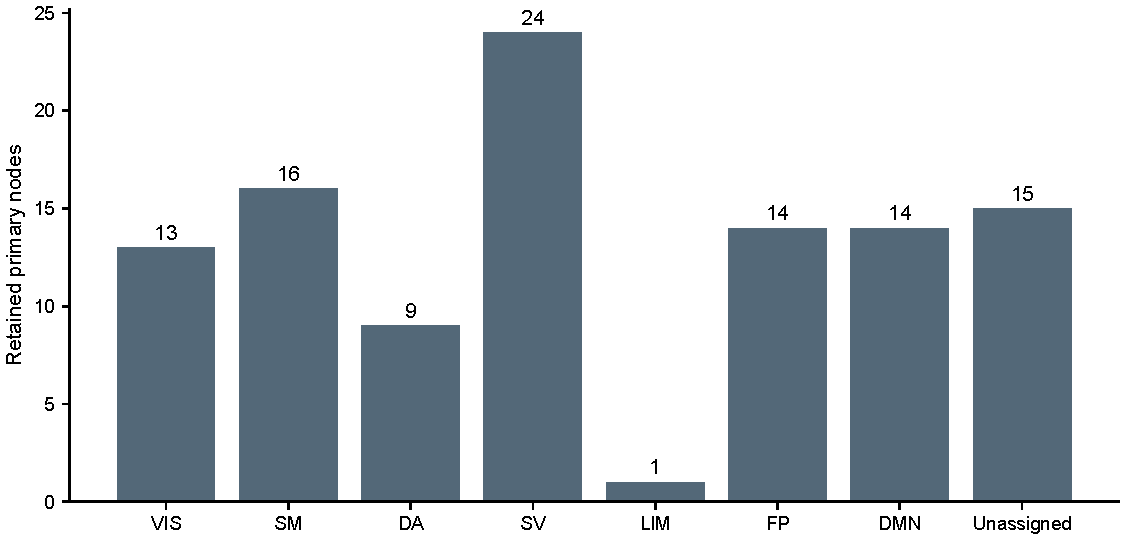
\includegraphics[width=.98\textwidth,height=.66\textheight,keepaspectratio]{figures/SFig1.pdf}
\caption{\textbf{Composition of the primary node set.} The common 106-node graph contains 91 cortical-assigned and 15 unassigned nodes. The seven network counts are shown. A single limbic node cannot support within-network edges.}\label{sfig:1}
\end{figure}
\clearpage

Figure~\ref{sfig:2} presents raw h estimates across node-set designs.
\begin{figure}[H]
\centering
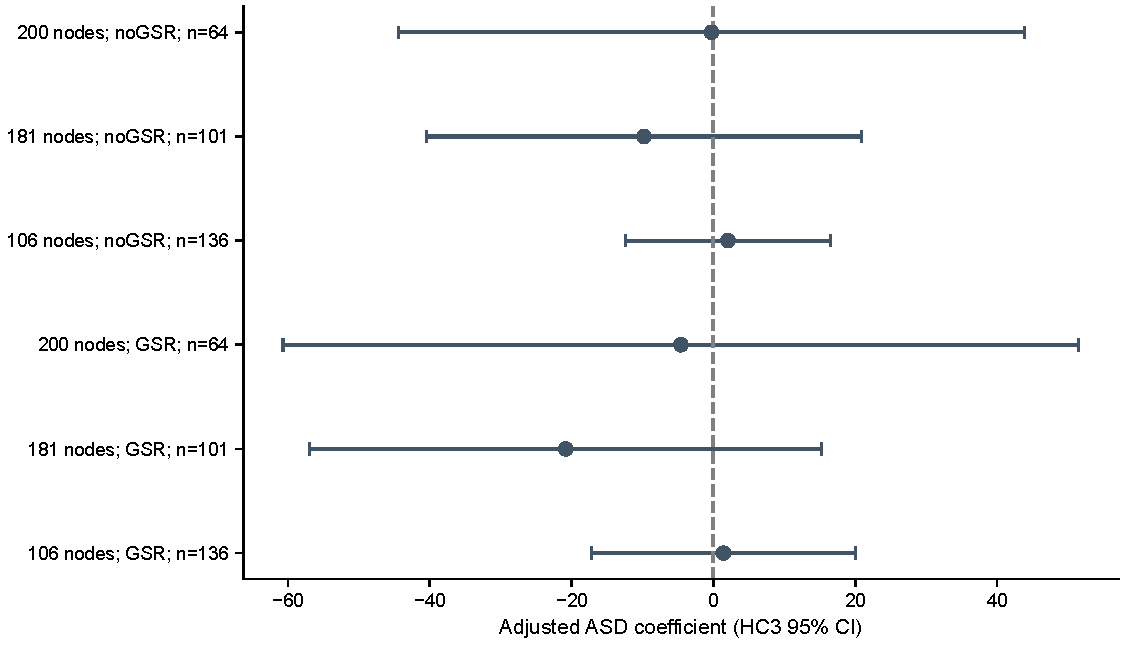
\includegraphics[width=.98\textwidth,height=.66\textheight,keepaspectratio]{figures/SFig2.pdf}
\caption{\textbf{Raw H estimates across node-set designs.} Points show adjusted diagnosis coefficients and HC3 95\% intervals. Node and participant sets differ across designs; these comparisons cannot isolate a node-count effect.}\label{sfig:2}
\end{figure}
\clearpage

Figure~\ref{sfig:3} presents individual male-control empirical and null energies.
\begin{figure}[H]
\centering
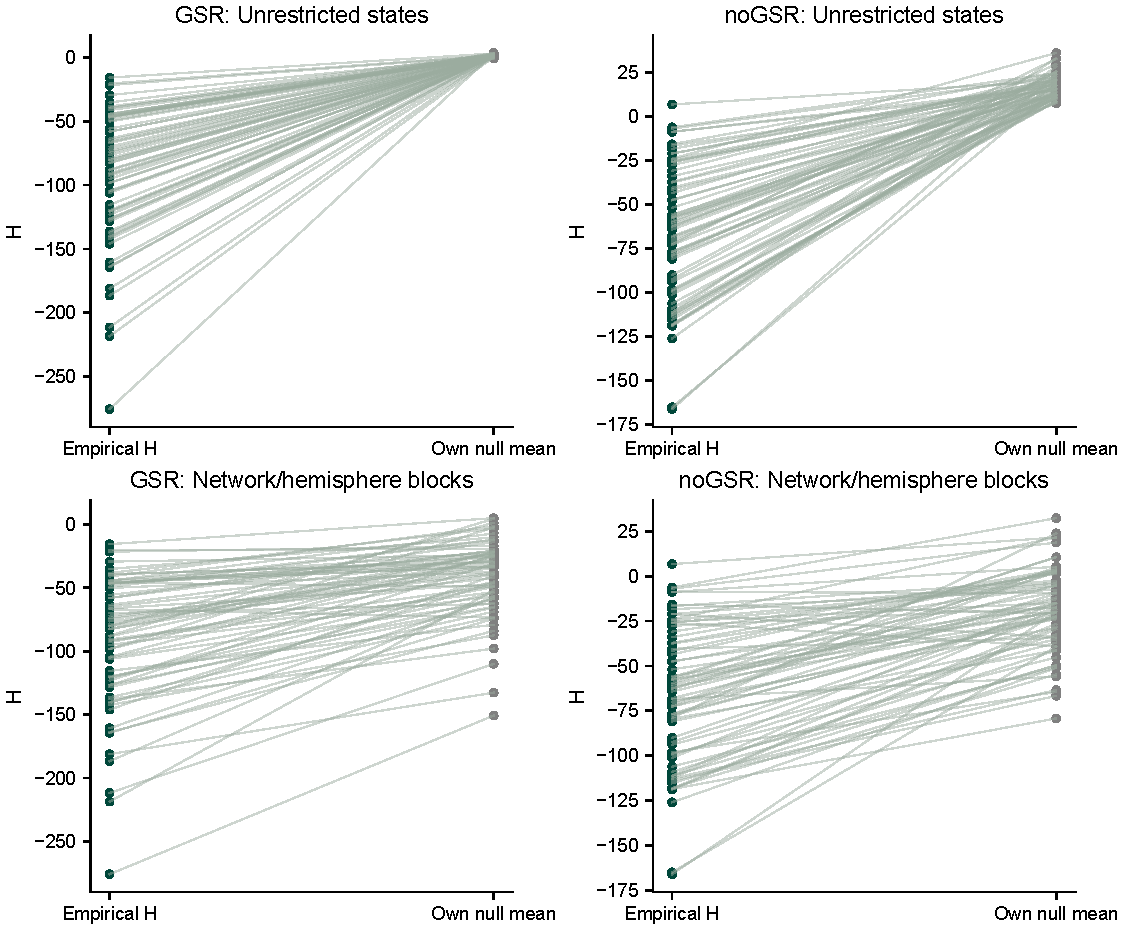
\includegraphics[width=.98\textwidth,height=.66\textheight,keepaspectratio]{figures/SFig3.pdf}
\caption{\textbf{Individual male-control empirical and null energies.} Each line connects the empirical H of one of 71 controls to that participant's mean of 1,000 randomizations. Pipelines and null constraints are separated. No topology rewiring is performed.}\label{sfig:3}
\end{figure}
\clearpage

Figure~\ref{sfig:4} presents participant-level null z-scores.
\begin{figure}[H]
\centering
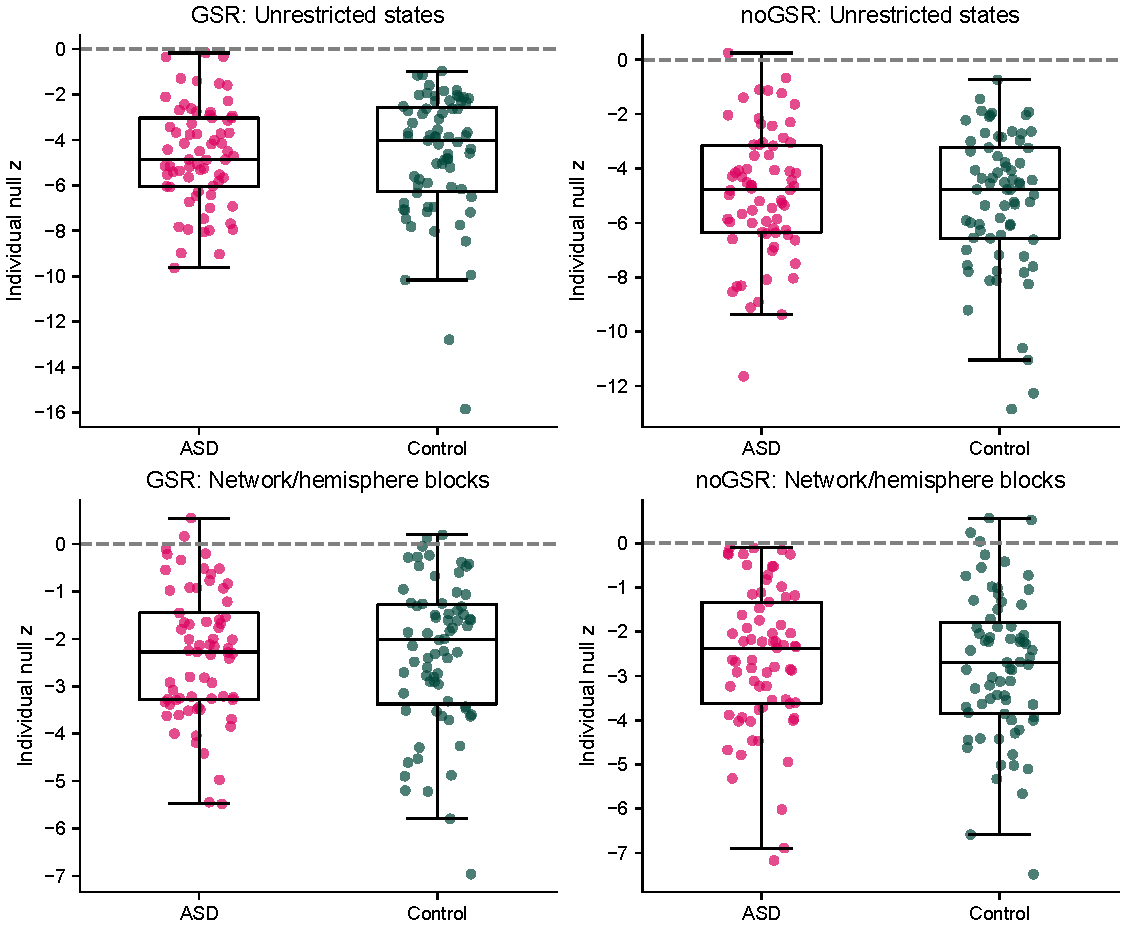
\includegraphics[width=.98\textwidth,height=.66\textheight,keepaspectratio]{figures/SFig4.pdf}
\caption{\textbf{Participant-level null z-scores.} Both groups are shown under unrestricted and blocked state permutations. Negative z denotes H below the individual null mean. These are alignment comparisons, not diagnosis tests.}\label{sfig:4}
\end{figure}
\clearpage

Figure~\ref{sfig:5} presents within-network block-energy distributions.
\begin{figure}[H]
\centering
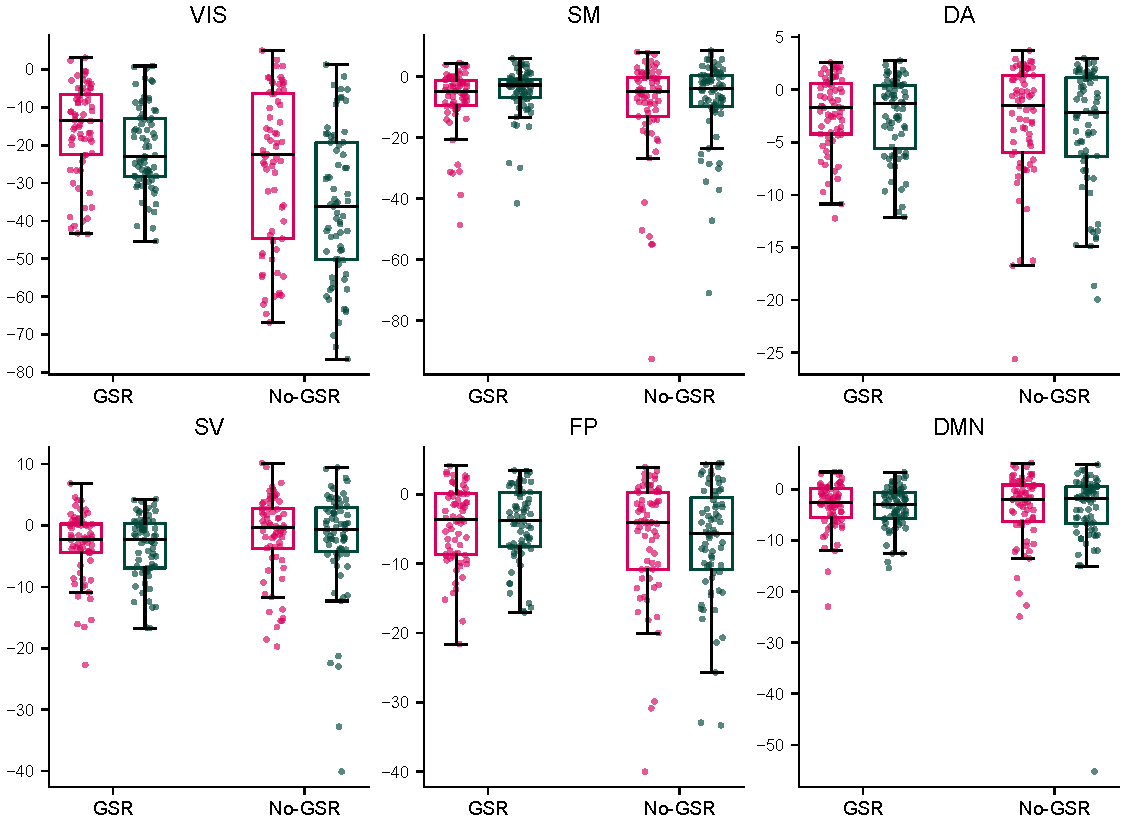
\includegraphics[width=.98\textwidth,height=.66\textheight,keepaspectratio]{figures/SFig5.pdf}
\caption{\textbf{Within-network block-energy distributions.} All six available within-network energy blocks are shown in both pipelines. ASD is magenta and controls dark green. Descriptive distributions use all 140 eligible participants, whereas adjusted comparisons use 136.}\label{sfig:5}
\end{figure}
\clearpage

Figure~\ref{sfig:6} presents baseline classifier confusion matrices.
\begin{figure}[H]
\centering
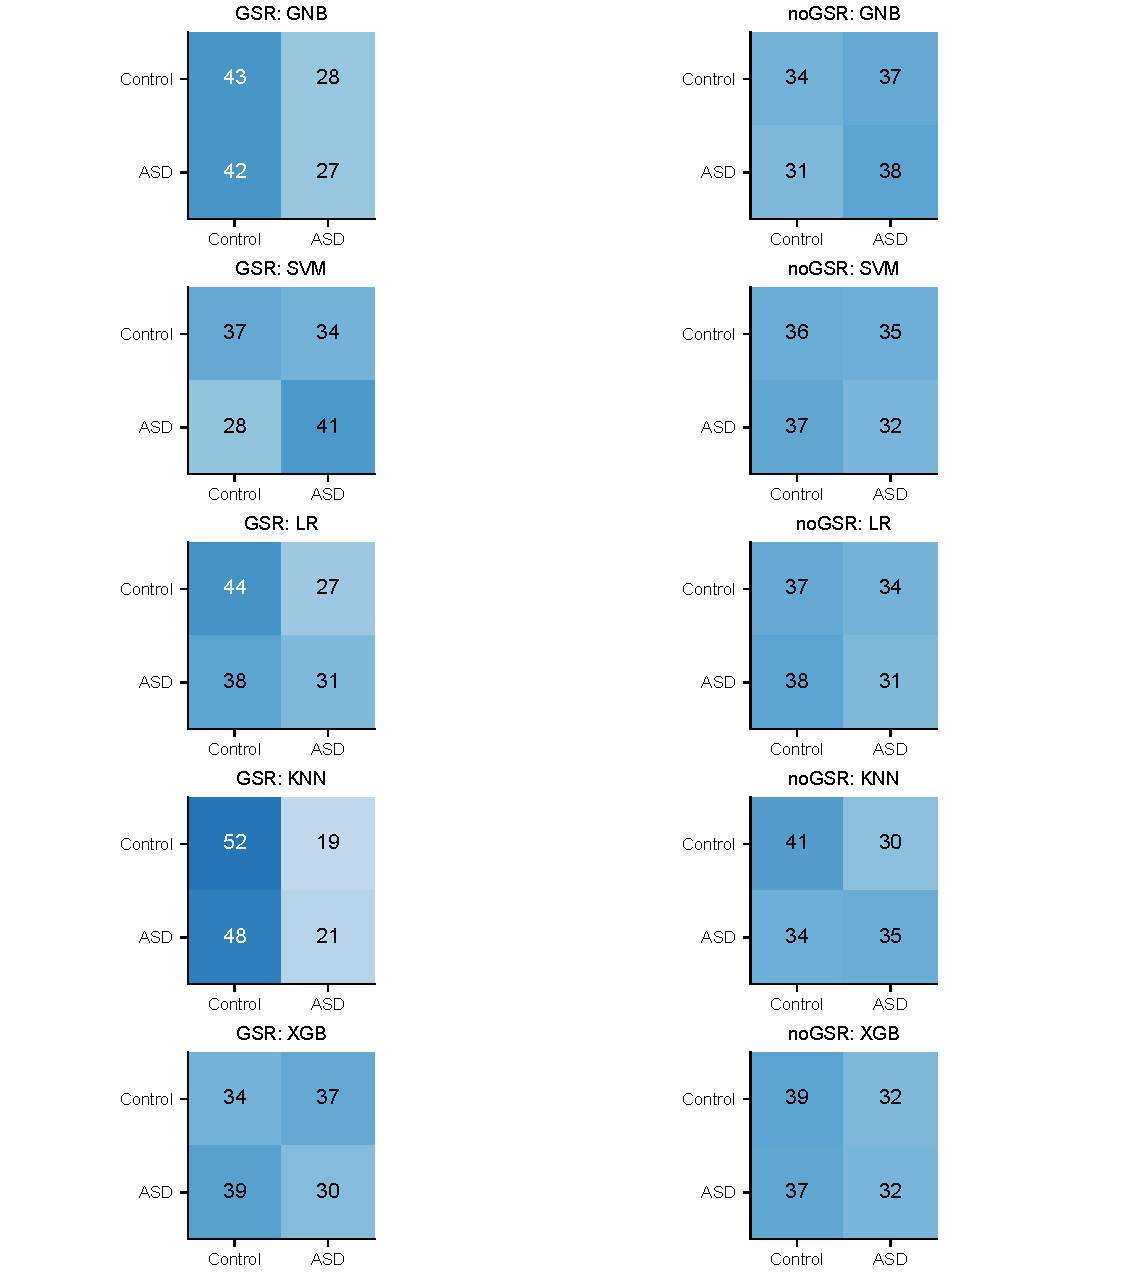
\includegraphics[width=.98\textwidth,height=.66\textheight,keepaspectratio]{figures/SFig6.pdf}
\caption{\textbf{Baseline classifier confusion matrices.} Each matrix contains all 140 complete out-of-fold predictions. Counts are printed and color encodes true-class-normalized proportions for every model and pipeline. No model is selected from outer-fold performance.}\label{sfig:6}
\end{figure}
\clearpage

Figure~\ref{sfig:7} presents descriptive principal-component projection.
\begin{figure}[H]
\centering
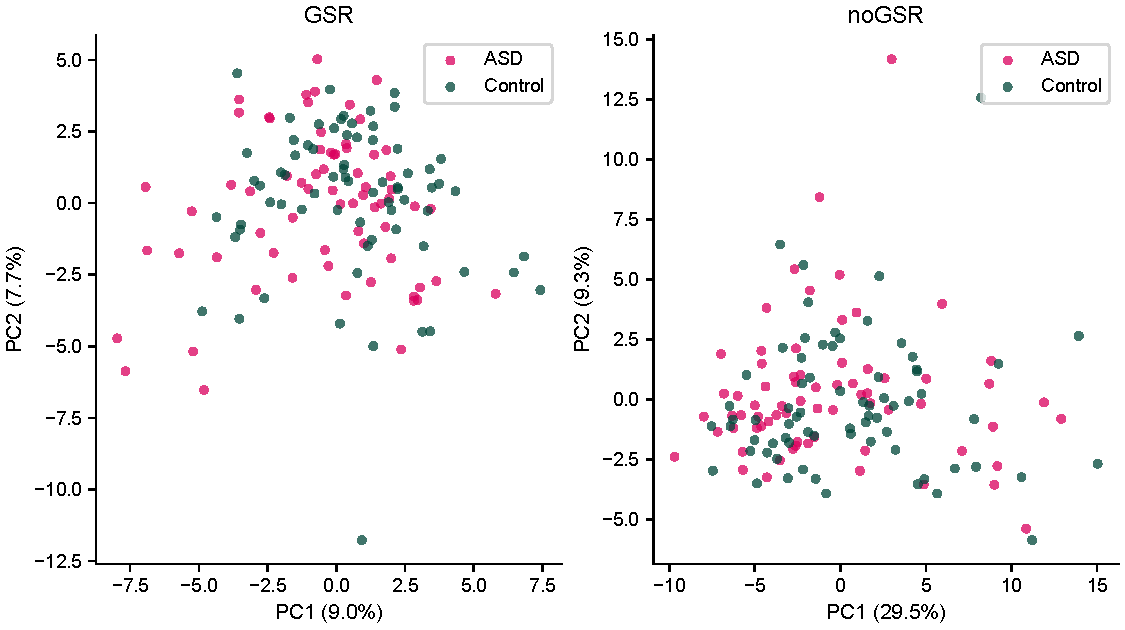
\includegraphics[width=.98\textwidth,height=.66\textheight,keepaspectratio]{figures/SFig7.pdf}
\caption{\textbf{Descriptive principal-component projection.} PCA uses the standardized raw common 88-feature matrix and all 140 participants separately per pipeline. ASD is magenta and controls dark green. This full-sample descriptive projection is not used in cross-validation, feature selection or inferential testing. Projection coordinates are in S2 Data.}\label{sfig:7}
\end{figure}
\clearpage

Figure~\ref{sfig:8} presents exploratory feature-selection performance comparison.
\begin{figure}[H]
\centering
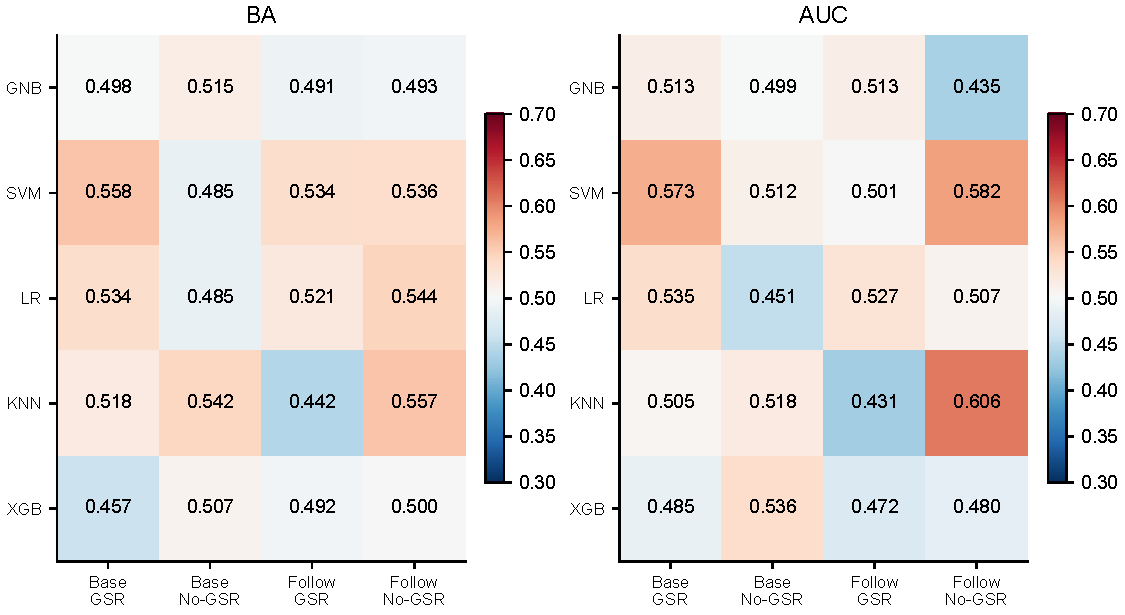
\includegraphics[width=.98\textwidth,height=.66\textheight,keepaspectratio]{figures/SFig8.pdf}
\caption{\textbf{Exploratory feature-selection performance comparison.} Balanced accuracy and ROC AUC are shown for every baseline and follow-up model/pipeline pair. The follow-up was specified after baseline outer performance was known and is exploratory.}\label{sfig:8}
\end{figure}
\clearpage

Figure~\ref{sfig:9} presents exploratory feature-selection roc curves.
\begin{figure}[H]
\centering
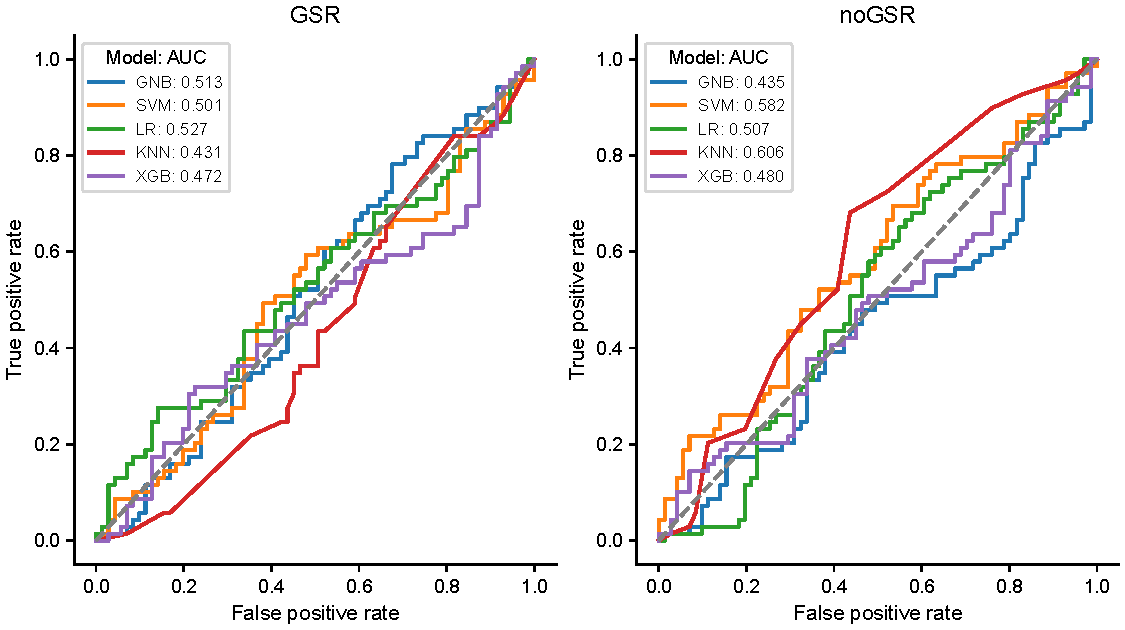
\includegraphics[width=.98\textwidth,height=.66\textheight,keepaspectratio]{figures/SFig9.pdf}
\caption{\textbf{Exploratory feature-selection ROC curves.} All models use complete out-of-fold scores and the same known outer site folds. A better point estimate does not constitute independent confirmation of improvement.}\label{sfig:9}
\end{figure}
\clearpage

Figure~\ref{sfig:10} presents exploratory feature-selection confusion matrices.
\begin{figure}[H]
\centering
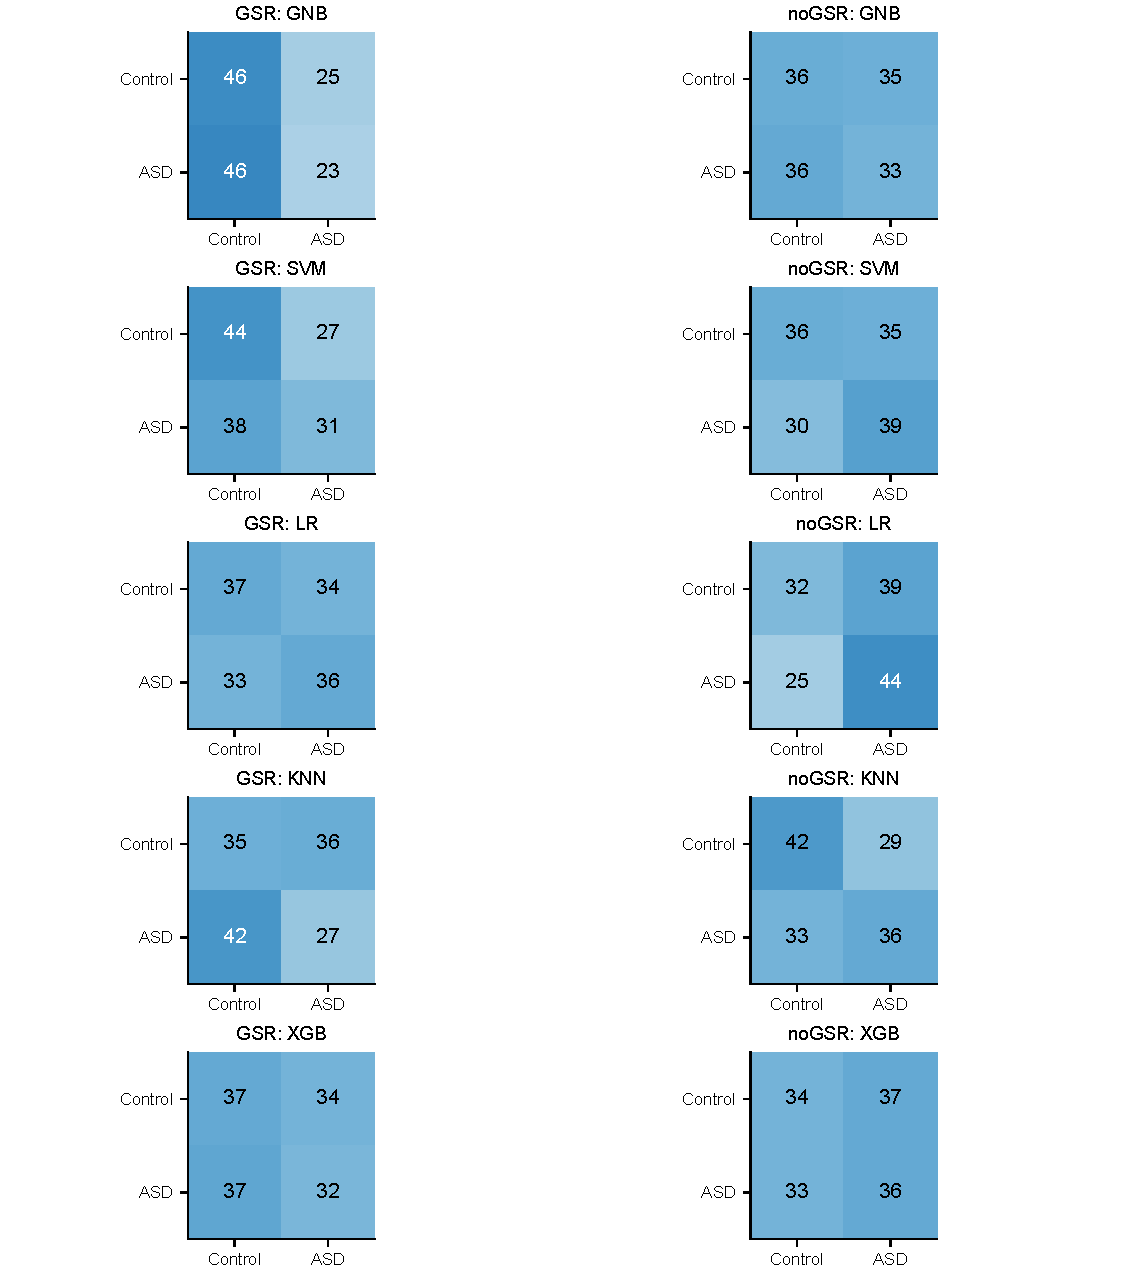
\includegraphics[width=.98\textwidth,height=.66\textheight,keepaspectratio]{figures/SFig10.pdf}
\caption{\textbf{Exploratory feature-selection confusion matrices.} Counts are printed and color encodes row-normalized proportions, using all 140 out-of-fold predictions per model/pipeline pair. Selection and fitting occur inside training folds.}\label{sfig:10}
\end{figure}
\clearpage

Figure~\ref{sfig:11} presents baseline feature-selection frequencies.
\begin{figure}[H]
\centering
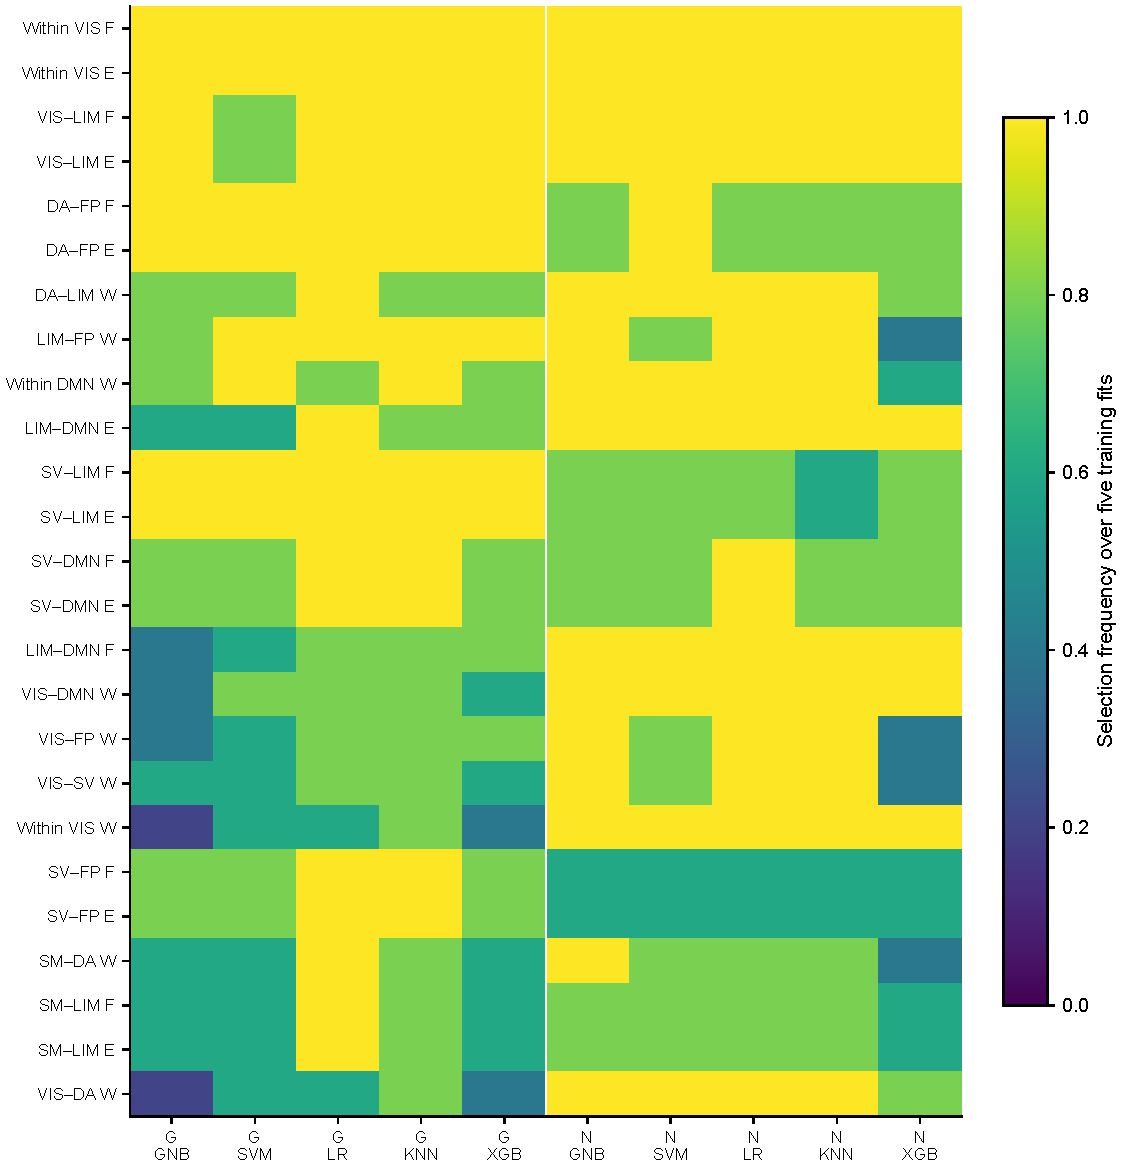
\includegraphics[width=.98\textwidth,height=.66\textheight,keepaspectratio]{figures/SFig11.pdf}
\caption{\textbf{Baseline feature-selection frequencies.} The 25 most frequently retained features per pipeline are shown across five overlapping outer training sets for each model. Frequencies describe selection, not significance, coefficient magnitude or causal relevance. Full selected names are in S2 Data.}\label{sfig:11}
\end{figure}
\clearpage

Figure~\ref{sfig:12} presents follow-up feature-selection frequencies.
\begin{figure}[H]
\centering
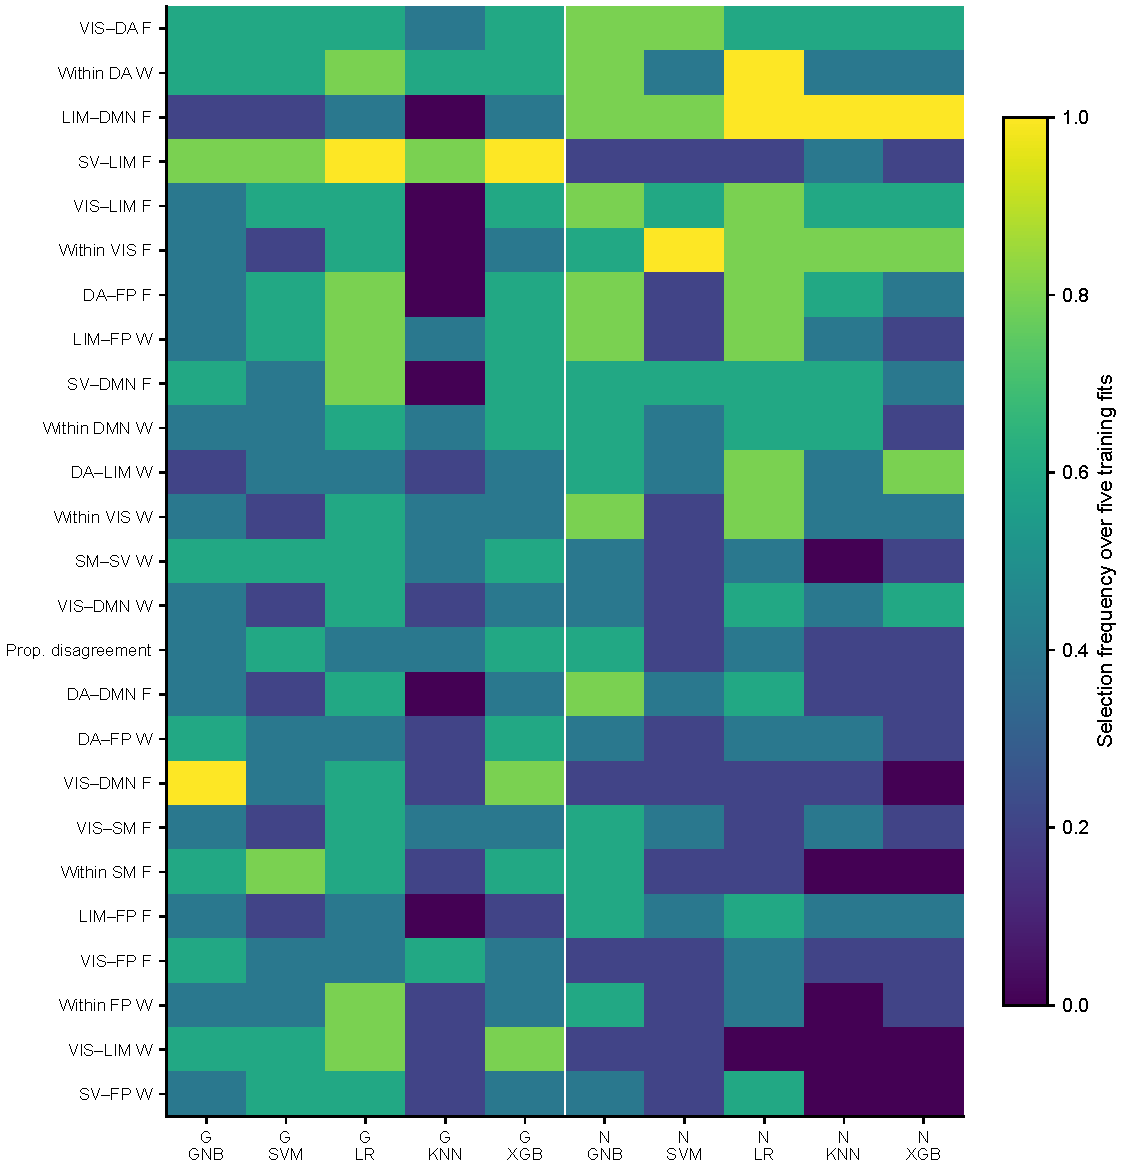
\includegraphics[width=.98\textwidth,height=.66\textheight,keepaspectratio]{figures/SFig12.pdf}
\caption{\textbf{Follow-up feature-selection frequencies.} The top 25 features are ranked by total retained frequency across model fits. Training-only redundancy pruning precedes the chosen selector. Overlapping folds and multiple procedures preclude interpreting frequencies as independent biomarker evidence.}\label{sfig:12}
\end{figure}
\clearpage

Figure~\ref{sfig:13} presents plsc latent covariance summaries.
\begin{figure}[H]
\centering
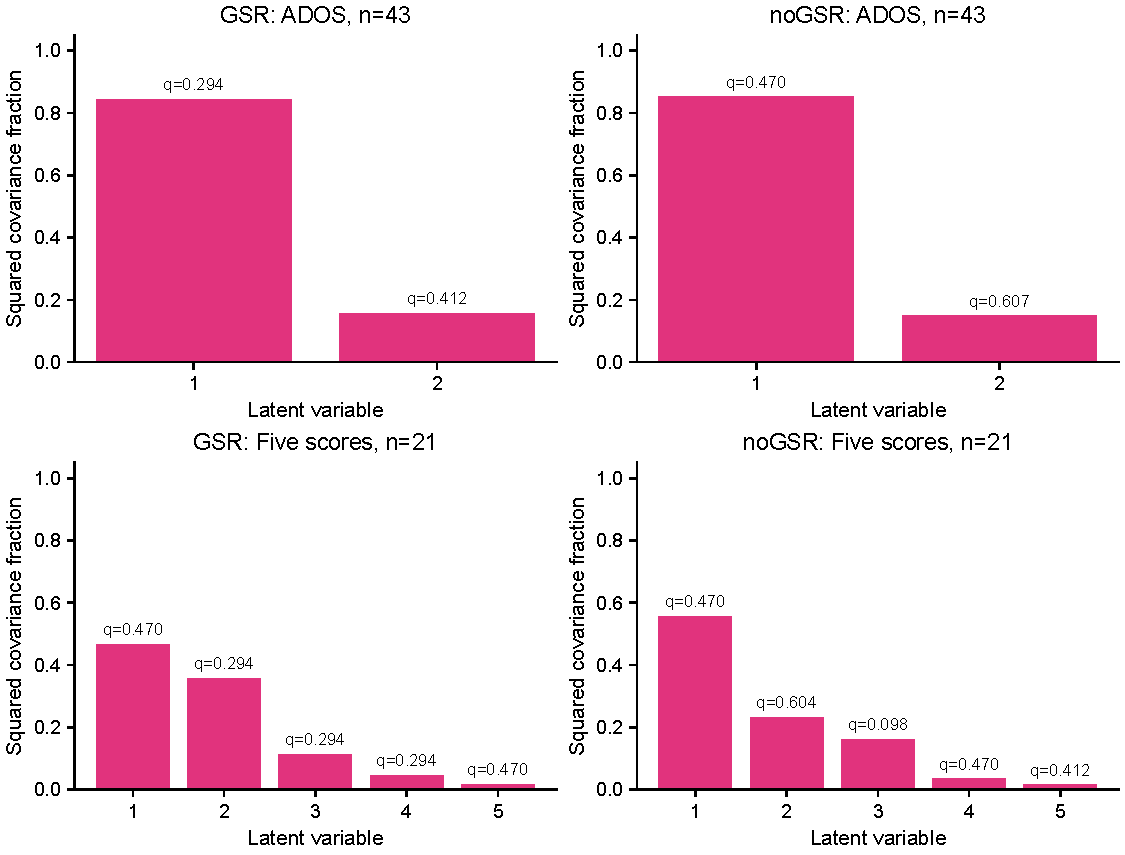
\includegraphics[width=.98\textwidth,height=.66\textheight,keepaspectratio]{figures/SFig13.pdf}
\caption{\textbf{PLSC latent covariance summaries.} Squared singular-value fractions and corrected rank-wise permutation probabilities are shown for ADOS and five-score complete-case blocks. Sample sizes are 43 and 21. No latent-variable test survives BH across the 14 tests; covariance fractions are not out-of-sample predictive accuracy.}\label{sfig:13}
\end{figure}
\clearpage
\end{document}
